\documentclass[12pt]{article}
\usepackage[english]{babel}
\usepackage{natbib}
\usepackage{url}
\usepackage[utf8x]{inputenc}
\usepackage{amsmath}
\usepackage{graphicx}
\usepackage{parskip}
\usepackage{fancyhdr}
\usepackage{vmargin}
\setmarginsrb{3 cm}{2.5 cm}{3 cm}{2.5 cm}{1 cm}{1.5 cm}{1 cm}{1.5 cm}

\title{Atmosfera de la tierra}								% Title
\author{Martha Anahí Iñiguez Beltrán}						% Author
\date{\today}											% Date

\makeatletter
\let\thetitle\@title
\let\theauthor\@author
\let\thedate\@date
\makeatother

\pagestyle{fancy}
\fancyhf{}
\rhead{Física Computacional}
\lhead{\thetitle}
\cfoot{\thepage}

\begin{document}

\begin{titlepage}
\centering
    \vspace*{0.5 cm}
    \textsc{\LARGE Universidad de Sonora}\\[2.0 cm]	% University Name
    \textsc{\Large Departamento de ciencias exactas}\\[1.0 cm]
\textsc{\Large Física Computacional}\\[0.5 cm]
\rule{\linewidth}{0.2 mm} \\[0.4 cm]
{ \huge \bfseries \thetitle}\\
\rule{\linewidth}{0.2 mm} \\[1.5 cm]
\begin{minipage}{0.6\textwidth}
\begin{flushleft} \large
\emph{Alumno:}\\
\theauthor
\end{flushleft}
\end{minipage}~
\begin{minipage}{0.4\textwidth}
\begin{flushright} \large
\end{flushright}
\end{minipage}\\[2 cm]


{\large \thedate}\\[2 cm]

\vfill

\end{titlepage}

%%%%%%%%%%%%%%%%%%%%%%%%%%%%%%%%%%%%%%%%%%%%%%%%%%%%%%%%%%%%%%%%%%%%%%%%%%%%%%%%%%%%%%%%%

\tableofcontents
\pagebreak


\section{Introducción}
\noindent

La atmósfera de la Tierra es la capa de gases, comúnmente conocida como aire , que rodea al planeta Tierra y es retenida por la gravedad de la Tierra . La atmósfera de la Tierra protege la vida en la Tierra creando presión permitiendo que exista agua líquida en la superficie de la Tierra , absorbiendo radiación solar ultravioleta , calentando la superficie mediante retención de calor ( efecto invernadero ) y reduciendo las temperaturas extremas entre el día y la noche (la temperatura diurna variación ).

Por volumen, el aire seco contiene 78.09\% de nitrógeno , 20.95\% de oxígeno , 0.93\% de argón , 0.04\% de dióxido de carbono y pequeñas cantidades de otros gases. El aire también contiene una cantidad variable de vapor de agua , en promedio alrededor de 1\% a nivel del mar, y 0.4\% en toda la atmósfera. El contenido de aire y la presión atmosférica varían en las diferentes capas, y el aire adecuado para su uso en la fotosíntesis por plantas terrestres y la respiración de animales terrestres se encuentra solo en la troposfera terrestre y en atmósferas artificiales .

\begin{figure}
  \begin{centering}
  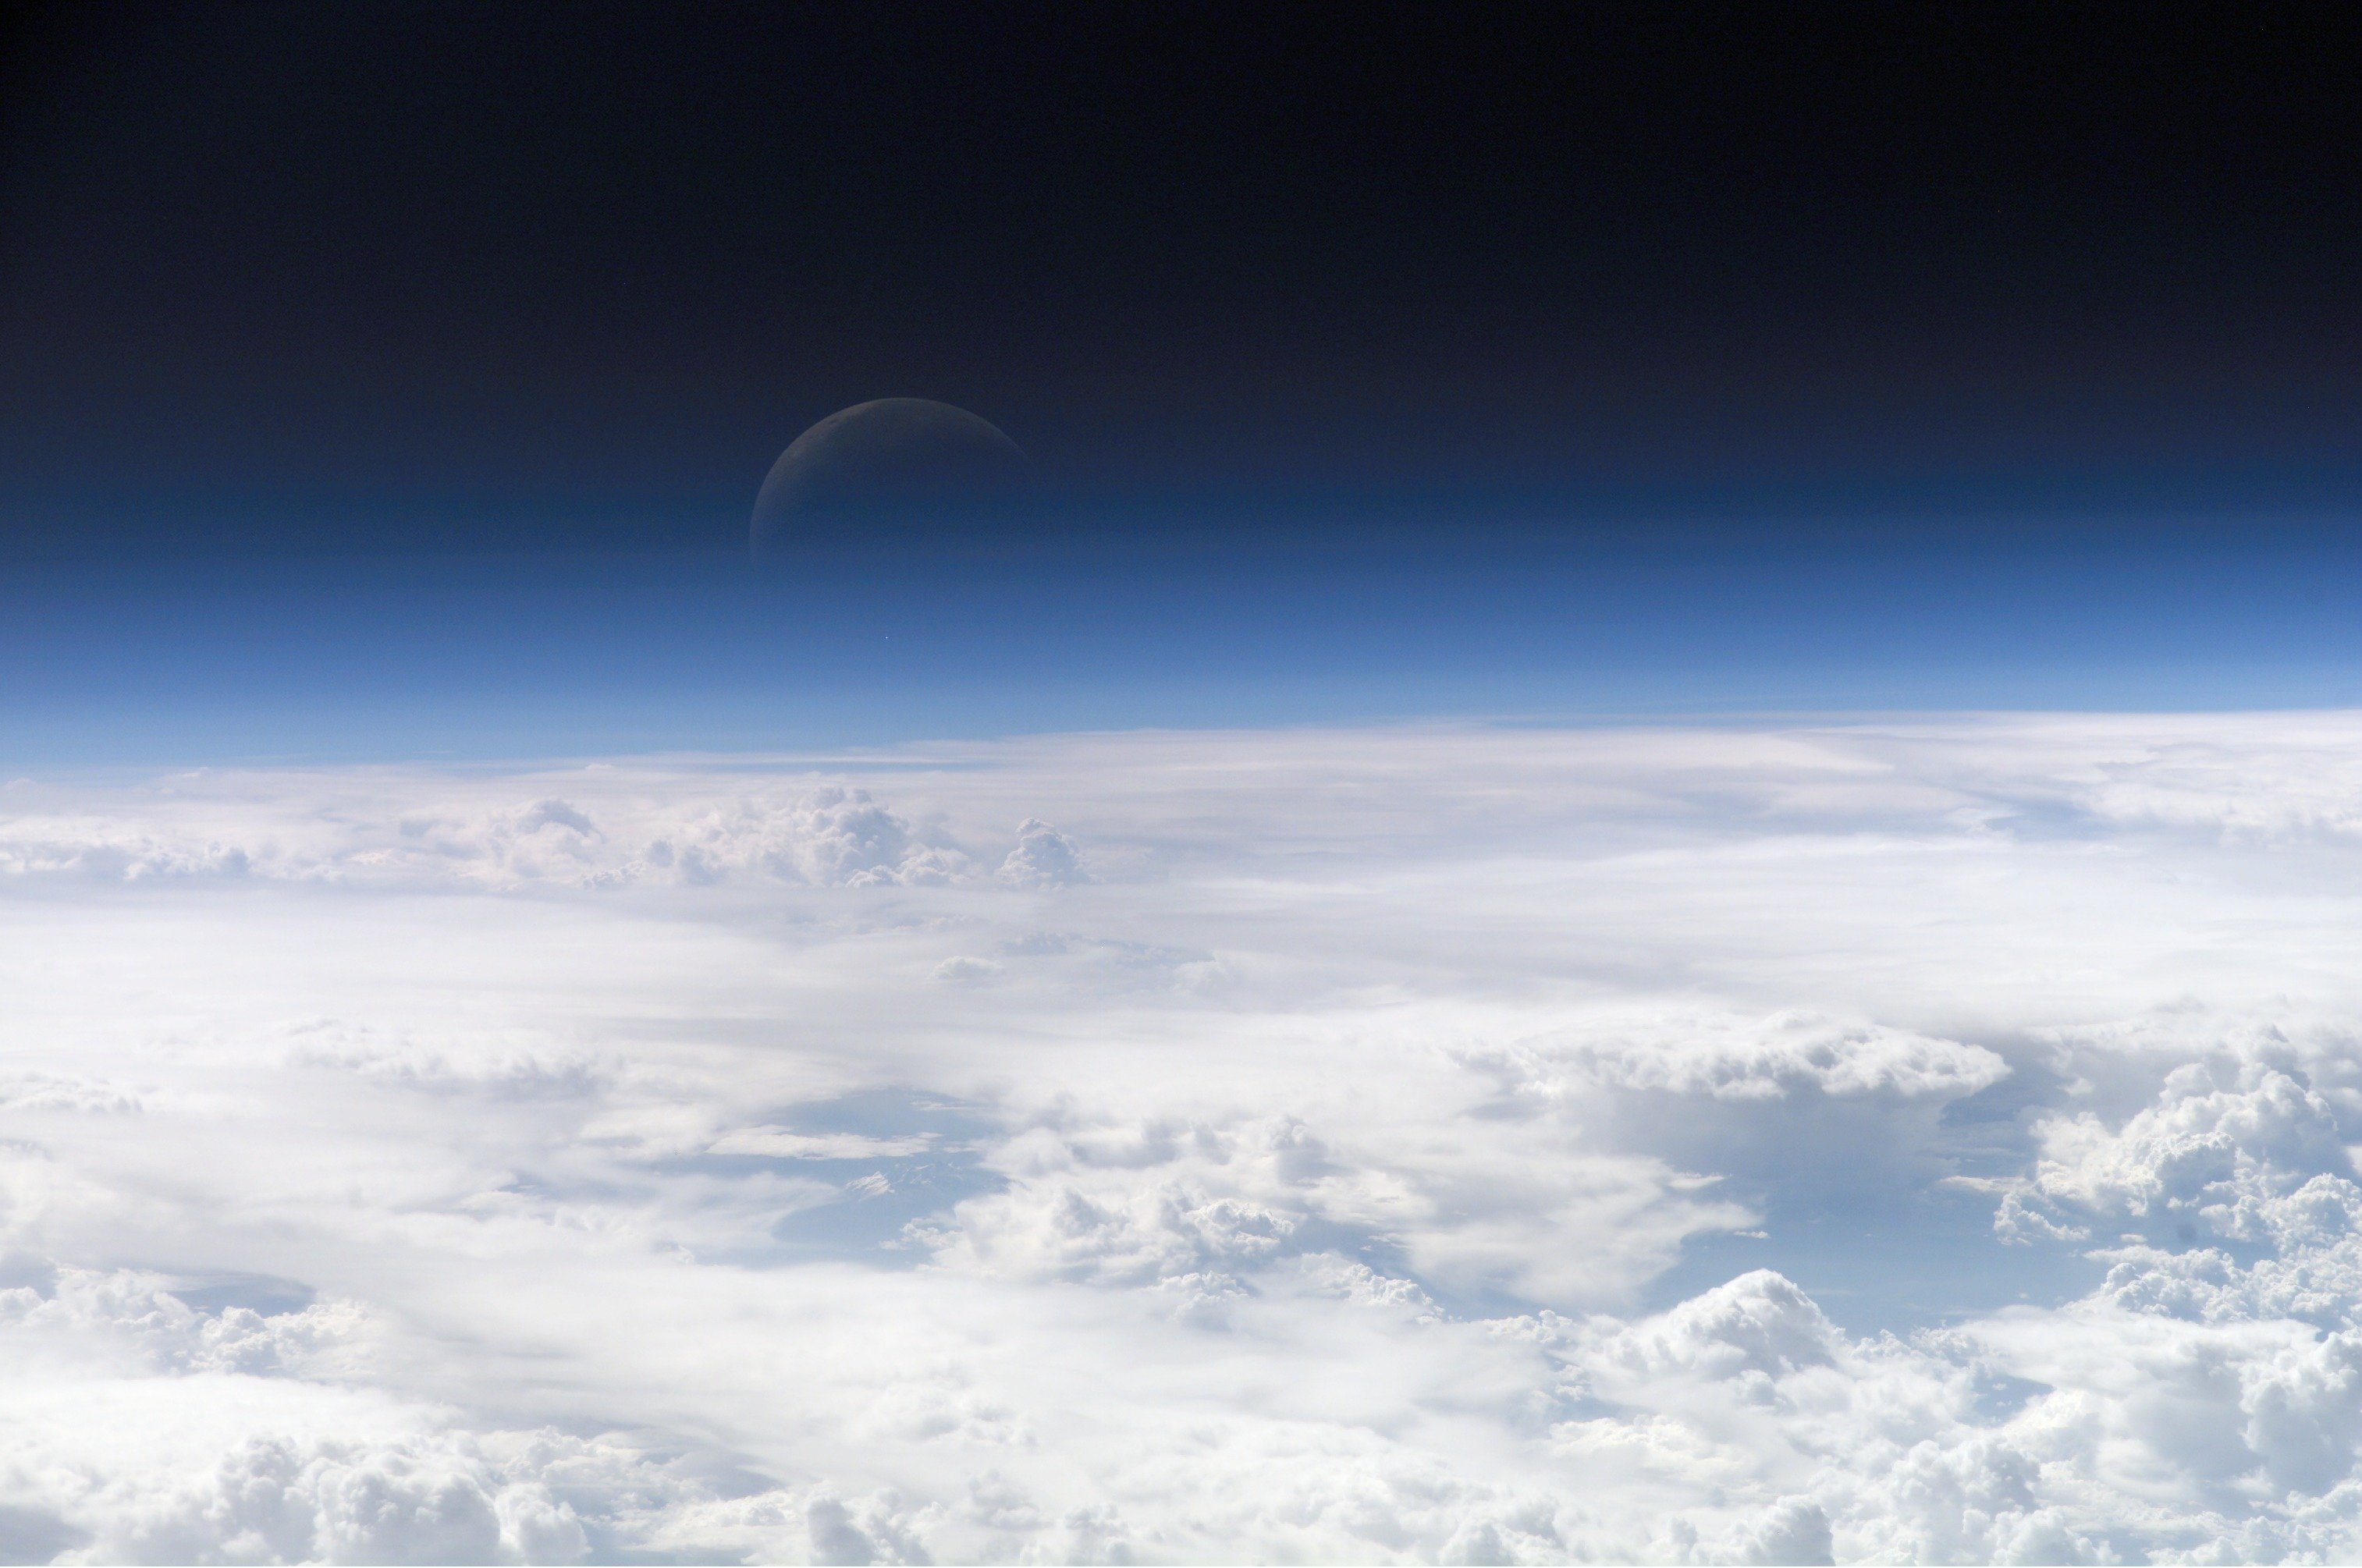
\includegraphics[scale = 0.09]{Top_of_Atmosphere.jpg}
  \caption{Figura 1: Cima de la atmósfera}
  \end{centering}
\end{figure}

\section{Composición}

Los tres mayores constituyentes de el aire, y por lo tanto de la atmósfera, son Nitrógeno, Oxígeno y Argón. El vapor de agua aporta aproximadamente el 0.25\% de la masa de la atmósfera. La concentración de gas invernadero varía significativamente alrededor de 10 ppm por el volumen de las porciones más frías de la atmósfera hasta 5\% del volumen en las más calientes, masas de aire húmedo y concentraciones de otros gases atmosféricos que se denominan en términos de aire seco. Los gases restantes a menudo se denominan como gases traza, los cuales son gas invernadero, principalmente dióxido de carbono, metano, oxido nitroso y ozono. El aire filtrado incluye pequeñas cantidades de muchos otros compuestos químicos. Muchas sustancias de orígen natural pueden presentar local y estacionalmente pequeñas cantidades de aerosol en muestras de aire no filtrado, incluyendo polvo de composición orgánica y mineral, polen y esporas, rocío de mar y cenizas volcánicas. Varios contaminantes industriales puedes estar presentes támbien en forma de gases o aerosoles, como cloro, compuestos de flúor y vapor de mercurio elemental. Compuestos de azufre tales como el sulfuro de hidrógeno y dióxido de azufre se pueden derivar de la contaminación del aire industrial.

\section{Estructura de la Atmósfera}

\begin{figure}
  \begin{centering}
  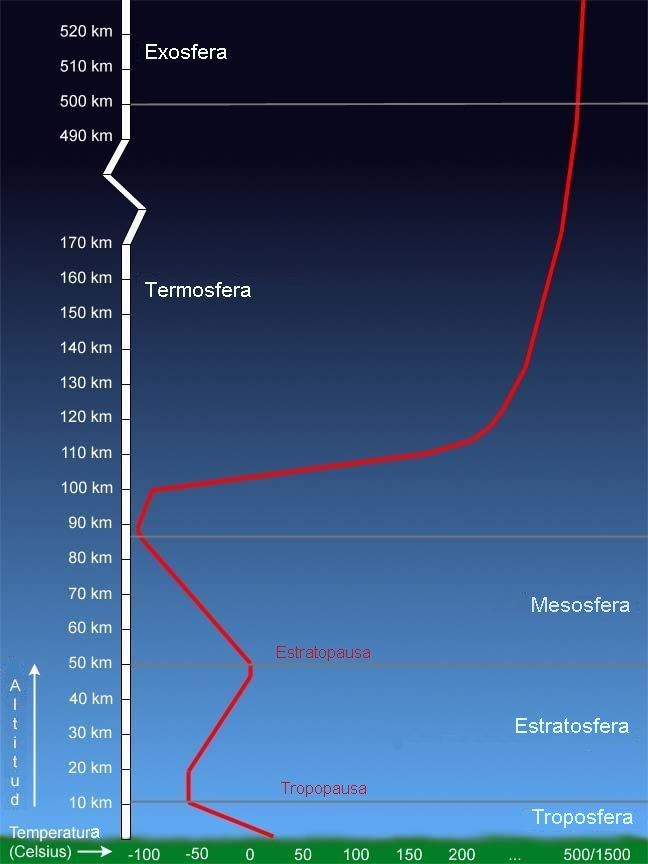
\includegraphics[scale = 0.3]{capesatmosfera.jpg}
  \caption{Figura 1: Estructura de la atmósfera}
  \end{centering}
\end{figure}


En general, la presión del aire y la densidad disminuyen con la altitud en la atmósfera. Sin embargo, la temperatura tiene un perfil más complicado con la altitud y puede permanecer relativamente constante o incluso aumentar en algunas regiones. Debido a que el patrón general del perfil de la temperatura-altitud es constante y medible por medio de sondeos de globo instrumentados, el comportamiento de la temperatura proporciona una medida útil para distinguir las capas atmosféricas. De esta manera, la atmósfera terrestre se puede dividir en cinco capas principales. Excluyendo la exosfera, la atmósfera tiene cuatro capas principales, que son la troposfera, la estratosfera, la mesosfera y la termosfera. De mayor a menor, las cinco capas principales son:

- Exosfera: 700 a 10,000 km \\- Termosfera: 80 a 700 km \\- Mesosfera: 50 a 80 km \\- Estratosfera: 12 a 50 km\\- Troposfera: 0 a 12 km

\subsection{Exosfera}

La exosfera es la capa más externa de la atmósfera terrestre, es decir, el límite superior de la atmósfera. Se extiende desde la exobase, que se encuentra en la parte superior de la termosfera a una altitud de aproximadamente de 700 km sobre el nivel del mar, a unos 10 000 km donde se funde el viento solar.

Esta capa está compuesta principalmente de densidades extremadamente bajas de hidrógeno, helio y varias moléculas más pesadas, incluyendo nitrógeno, oxígeno y dióxido de carbono más cerca de la exobase. Los átomos y las moléculas están tan separados que pueden viajar cientos de kilómentros sin colisionar entre sí. Por lo tanto, la exosfera ya no se comporta como un gas y las partículas escapan constantemente al espacio. Estas partículas que se mueven libremente siguen trayectorias balísticas y pueden migrar dentro y fuera de la magnetosfera o del viento solar.

La exosfera está ubicada muy por encima de la tierra para que sea posible cualquier fenómeno meteorológico. Sin embargo, la aurora boreal y la aurora austral a veces se encuentran en la parte inferior de la exosfera, donde se superponen a la termósfera. La exosfera contiene la mayoría de los satélites que orbitan alrededor de la tierra.

\subsection{Termósfera}

La termósfera es la segunda capa más alta de la atmósfera de la Tierra. Se extiende desde la mesopausia, que lo separa de la mesósfera, a una altitud de 80 km hasta la termopausia en un rango de altitud de 500 a 1000 km. La altura de la termopausia varía considerablemente debido a los cambios en la actividad solar. Debido a que la termopausia se encuentra en el límite inferior de la exósfera, que es también referido como la exobase. La parte inferior de la termósfera, de 80 a 550 km sobre la superficie terrestre, contiene la ionosfera.

La temperatura de la termósfera aumenta gradualmente con la altura. A diferencia de la estratosfera, en donde la inversión de la temperatura se debe a la absorción de radiació por el ozono, la inversión en la termósfera  ocurre debido a la extremadamente baja densidad de sus moléculas. La temperatura de esta capa puede elevarse hasta 1500 grados Centígrados, aunque las moléculas de gas están tan separadas que su temperatura en el sentido habitual no es muy significativa. El aire está tan enrarecido que una molécula individual, oxígeno por ejemplo,  viaja un promedio de 1 km entre colisiones con otras moléculas. Aunque la termósfera tiene una alta proporción de moléculas con alta energía, no estaría caliente para un humano en contacto directo, ya que su densidad es demasiado baja para conducir una cantidad significativa de energía hacia o desde la piel.

Esta capa está completamente despejada y libre de vapor de agua. Sin embargo, fenómenos no hidrometeorológicos como la aurora boreal y la aurora austral se ven ocasionalmente en la termósfera. La Estación Espacial Internacional orbita en esta capa, entre 350 y 420 km.

\subsection{Mesósfera}

La mesosfera es la tercera capa más alta de la atmósfera de la Tierra, ocupando la región sobre la estratosfera y debajo de la termosfera. Se extiende desde la estrapaso a una altitud de aproximadamente 50 km a la mesoopausia a 80-85 km sobre el nivel del mar.

Las temperaturas caen con el aumento de la altitud a la mesopausia que marca la parte superior de esta capa media de la atmósfera. Es el lugar más frío de la Tierra y tiene una temperatura promedio de alrededor de -85 grados centígrados.

Justo debajo de la mesopausia, el aire es tan frío que incluso el vapor de agua, muy escaso en esta altitud, se puede sublimar en nubes noctiluces mesosféricas polares . Estas son las nubes más altas en la atmósfera y pueden ser visibles a simple vista si la luz del sol se refleja en ellas una o dos horas después de la puesta del sol o un período de tiempo similar antes del amanecer. Son más fácilmente visibles cuando el Sol está alrededor de 4 a 16 grados bajo el horizonte. Las descargas inducidas por rayos conocidas como eventos luminosos transitorios ocasionalmente se forman en la mesosfera por encima de las nubes de tormenta troposféricas . La mesosfera es también la capa donde la mayoría de los meteorosquemarse en la entrada atmosférica. Está demasiado elevado sobre la Tierra para que sea accesible para aviones y globos propulsados por aviones a reacción, y demasiado bajo para permitir naves espaciales orbitales. La mesosfera se accede principalmente por cohetes que suenan y aviones propulsados por cohetes.

\subsection{Estratosfera}

La estratosfera es la segunda capa más baja de la atmósfera de la Tierra. Se encuentra por encima de la troposfera y está separada de ella por la tropopausa . Esta capa se extiende desde la parte superior de la troposfera a aproximadamente 12 km de la superficie de la Tierra hasta la estratospausa a una altitud de aproximadamente 50 a 55 km.

La presión atmosférica en la parte superior de la estratosfera es aproximadamente 1/1000 de la presión al nivel del mar . Contiene la capa de ozono, que es la parte de la atmósfera de la Tierra que contiene concentraciones relativamente altas de ese gas. La estratosfera define una capa en la que las temperaturas aumentan con el aumento de la altitud. Este aumento de la temperatura es causado por la absorción de la radiación de la radiación ultravioleta del Sol por la capa de ozono , que restringe la turbulencia y la mezcla. Aunque la temperatura puede ser de -60 ° C (-76 ° F, 210 K) en la tropopausa, la parte superior de la estratosfera está mucho más caliente y puede estar cerca de 0 ° C.

El perfil de temperatura estratosférico crea condiciones atmosféricas muy estables, por lo que la estratosfera carece de la turbulencia del aire que produce el clima y que prevalece en la troposfera. En consecuencia, la estratosfera está casi completamente libre de nubes y otras formas de clima. Sin embargo, ocasionalmente se ven nubes polares estratosféricas o nacaradas en la parte inferior de esta capa de la atmósfera donde el aire es más frío. La estratosfera es la capa más alta a la que se puede acceder en aviones a reacción.

\subsection{Troposfera}

La troposfera es la capa más baja de la atmósfera de la Tierra. Se extiende desde la superficie de la Tierra hasta una altura promedio de aproximadamente 12 km, aunque esta altitud varía de unos 9 km en los polos a 17 km en el ecuador, con alguna variación debido al clima . La troposfera está delimitada por encima por la tropopausa , un límite marcado en la mayoría de los lugares por una inversión de temperatura (es decir, una capa de aire relativamente cálido por encima de uno más frío), y en otros por una zona que es isotérmica con la altura.

Aunque se producen variaciones, la temperatura generalmente disminuye con el aumento de la altitud en la troposfera porque la troposfera se calienta principalmente a través de la transferencia de energía desde la superficie. Por lo tanto, la parte más baja de la troposfera. La troposfera contiene aproximadamente el 80 \% de la masa de la atmósfera de la Tierra. La troposfera es más densa que todas las capas atmosféricas que la recubren porque un peso atmosférico más grande se encuentra en la parte superior de la troposfera y hace que se comprima más severamente. El cincuenta por ciento de la masa total de la atmósfera se encuentra en los 5,6 km más bajos de la troposfera.

Casi todo el vapor de agua atmosférico o humedad se encuentra en la troposfera, por lo que es la capa donde tiene lugar la mayor parte del clima de la Tierra. Básicamente tiene todos los tipos de nubes nubladas asociadas al clima generadas por la circulación activa del viento, aunque las nubes de trueno cumulonimbus muy altas pueden penetrar la tropopausa desde abajo y subir a la parte inferior de la estratosfera. La actividad de aviación más convencional tiene lugar en la troposfera, y es la única capa a la que se puede acceder mediante un avión propulsado por hélice.

\section{Propiedades Físicas}

\subsection{Presión y Espesor}

La presión atmosférica promedio a nivel del mar está definida por la Atmósfera Estándar Internacional como 101325 pascales. Esto a veces se conoce como una unidad de atmósferas estándar (atm) . La masa atmosférica total es 5.1480 × 10 a la 18 Kg aproximadamente un 2.5\% menos de lo que se deduciría de la presión media del nivel del mar y el área de la Tierra de 51007,2 megahectáreas, esta parte está desplazada por el terreno montañoso de la Tierra. La presión atmosférica es el peso total del aire sobre el área de la unidad en el punto donde se mide la presión. Por lo tanto, la presión del aire varía según la ubicación y el clima.  
\subsection{Temperatura y velocidad del sonido}

La división de la atmósfera en capas principalmente por referencia a la temperatura se discutió anteriormente. La temperatura disminuye con la altitud comenzando al nivel del mar, pero las variaciones en esta tendencia comienzan por encima de los 11 km, donde la temperatura se estabiliza a través de una gran distancia vertical a través del resto de la troposfera. En la estratosfera , comenzando por encima de unos 20 km, la temperatura aumenta con la altura, debido al calentamiento dentro de la capa de ozono causado por la captura de radiación ultravioleta significativa del Sol por el dioxígeno y el gas ozono en esta región. Todavía otra región de aumento de la temperatura con la altitud se produce a altitudes muy altas, en la termosfera acertadamente nombrada por encima de 90 km.

Debido a que en un gas ideal de composición constante, la velocidad del sonido depende únicamente de la temperatura y no de la presión o densidad del gas, la velocidad del sonido en la atmósfera con la altitud adquiere la forma del perfil de temperatura complicado (ver ilustración a la derecha) y no refleja los cambios altitudinales en densidad o presión.

%\begin{centering}
%\centering
%\begin{figure}
%  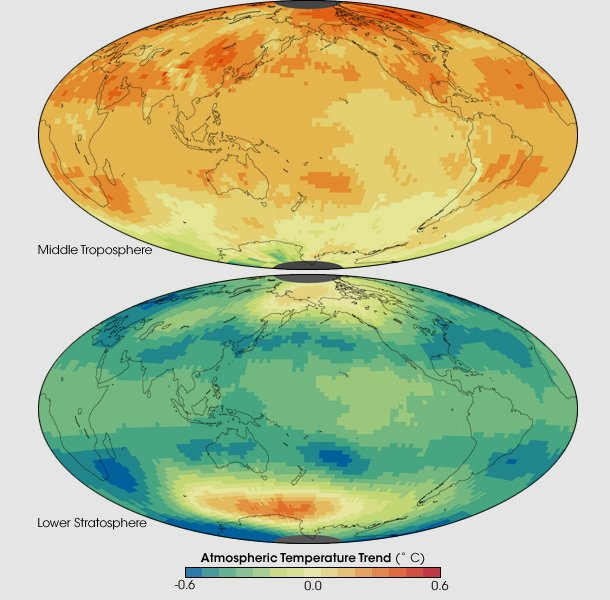
\includegraphics[scale = 0.4]{TEMPVEL.jpg}
%  \caption{Figura: Temperatura atmosférica}
%\end{figure}
%\end{centering}
%Agregar imágen temperatura

\subsection{Densidad y masa}

La densidad del aire a nivel del mar es de aproximadamente 1.2 kilogramos por metro cúbico. La densidad no se mide directamente, pero se calcula a partir de mediciones de temperatura, presión y humedad utilizando la ecuación de estado para el aire (una forma de la ley de los gases ideales ). La densidad atmosférica disminuye a medida que aumenta la altitud. Esta variación se puede modelar aproximadamente utilizando la fórmula barométrica . Se usan modelos más sofisticados para predecir la desintegración orbital de los satélites.

La masa promedio de la atmósfera es de aproximadamente 5 cuatrillones de toneladas o 1 / 1,200,000 la masa de la Tierra. Según el Centro Nacional Americano de Investigación Atmosférica , "la masa media total de la atmósfera es \[5.1480 × 10^{18} kg \] con un rango anual debido al vapor de agua de \[
1.2, 1.5 × 10^{15} kg \] dependiendo de si la presión de superficie o los datos de vapor de agua se utilizan, algo más pequeño que la estimación anterior. La masa media de vapor de agua se estima en \[ 1.27 × 10^{16} kg \] y la masa de aire seco es \[ 5.1352 ± 0.0003 × 10^{18} kg. \]

\section{Propiedades Ópticas}

La radiación solar (o luz solar) es la energía que la Tierra recibe del Sol . La Tierra también emite radiación hacia el espacio, pero a longitudes de onda más largas que no podemos ver. Parte de la radiación entrante y emitida es absorbida o reflejada por la atmósfera. En mayo de 2017, se descubrió que los reflejos de luz de los cristales de hielo en la atmósfera reflejaban destellos de luz, que se veían centellear desde un satélite en órbita a un millón de millas de distancia .

\subsection{Dispersión}

Cuando la luz pasa a través de la atmósfera de la Tierra, los fotones interactúan con ella a través de la dispersión . Si la luz no interactúa con la atmósfera, se llama radiación directa y es lo que verá si mirara directamente al Sol. La radiación indirecta es luz que se ha dispersado en la atmósfera. Por ejemplo, en un día nublado cuando no puedes ver tu sombra no hay radiación directa que te llegue, todo se ha dispersado. Como otro ejemplo, debido a un fenómeno llamado dispersión de Rayleigh, las longitudes de onda más cortas (azules) se dispersan más fácilmente que las longitudes de onda más largas (rojas). Es por eso que el cielo se ve azul; estás viendo luz azul dispersa. Esta es también la razón por la cual los atardeceres son rojos. Debido a que el Sol está cerca del horizonte, los rayos del Sol pasan a través de más atmósfera de la normal para llegar a su ojo. Gran parte de la luz azul se ha dispersado, dejando la luz roja en una puesta de sol.

\subsection{Absorción}

Diferentes moléculas absorben diferentes longitudes de onda de radiación. Por ejemplo, O2 y el ozono absorben casi todas las longitudes de onda de menos de 300 nanómetros . El agua (H2O) absorbe muchas longitudes de onda por encima de 700 nm. Cuando una molécula absorbe un fotón, aumenta la energía de la molécula. Esto calienta la atmósfera, pero la atmósfera también se enfría al emitir radiación, como se explica a continuación.

Los espectros de absorción combinados de los gases en la atmósfera dejan "ventanas" de baja opacidad , permitiendo la transmisión de solo ciertas bandas de luz. La ventana óptica se extiende desde alrededor de 300 nm (ultravioleta -C) hasta el rango que los humanos pueden ver, el espectro visible (comúnmente llamado luz), a aproximadamente 400-700 nm y continúa al infrarrojo a alrededor de 1100 nm. También hay ventanas de infrarrojos y de radio que transmiten algunas ondas infrarrojas y de radio a longitudes de onda más largas. Por ejemplo, la ventana de la radio va de aproximadamente un centímetro a ondas de aproximadamente once metros.

\subsection{Emisión}
La emisión es lo opuesto a la absorción, es cuando un objeto emite radiación. Los objetos tienden a emitir cantidades y longitudes de onda de radiación dependiendo de sus curvas de emisión de " cuerpo negro ", por lo tanto, los objetos más calientes tienden a emitir más radiación, con longitudes de onda más cortas. Los objetos más fríos emiten menos radiación, con longitudes de onda más largas. Por ejemplo, el Sol tiene aproximadamente 6.000  K (5.730° C ; 10.340° F ), su radiación alcanza un máximo de 500 nm y es visible para el ojo humano. La Tierra tiene aproximadamente 290 K (17° C; 62° F), por lo que su radiación alcanza un máximo cercano a las 10,000 nm, y es demasiado larga para ser visible para los humanos.

Debido a su temperatura, la atmósfera emite radiación infrarroja. Por ejemplo, en las noches despejadas, la superficie de la Tierra se enfría más rápido que en las noches nubladas. Esto se debe a que las nubes (H2O) son fuertes absorbedores y emisores de radiación infrarroja. Esta es también la razón por la cual se vuelve más fría por la noche en las elevaciones más altas.

El efecto invernadero está directamente relacionado con este efecto de absorción y emisión. Algunos gases en la atmósfera absorben y emiten radiación infrarroja, pero no interactúan con la luz solar en el espectro visible. Ejemplos comunes de estos son el dioxido de carbono y el agua.

\subsection{Índice de Refracción}

El índice de refracción del aire es cercano, pero apenas superior a 1. Las variaciones sistemáticas en el índice de refracción pueden conducir a la flexión de los rayos de luz en recorridos ópticos largos. Un ejemplo es que, en algunas circunstancias, los observadores a bordo de barcos pueden ver otras embarcaciones justo sobre el horizonte porque la luz se refracta en la misma dirección que la curvatura de la superficie de la Tierra.

El índice de refracción del aire depende de la temperatura, dando lugar a efectos de refracción cuando el gradiente de temperatura es grande. Un ejemplo de tales efectos es el espejismo .

\section{Circulación}

La circulación atmosférica (ver Figura) es el movimiento de aire a gran escala a través de la troposfera. Es el medio (junto con la circulación oceánica) por la cual el calor es distribuido al rededor de la tierra. La estructura de la circulación atmosférica varía año con año, pero la estructura básica se mantiene constante porque ésta es determinada por la tasa de rotación y la diferencia de radiación solar entre el ecuador y los polos.

\begin{figure}
\begin{centering}
  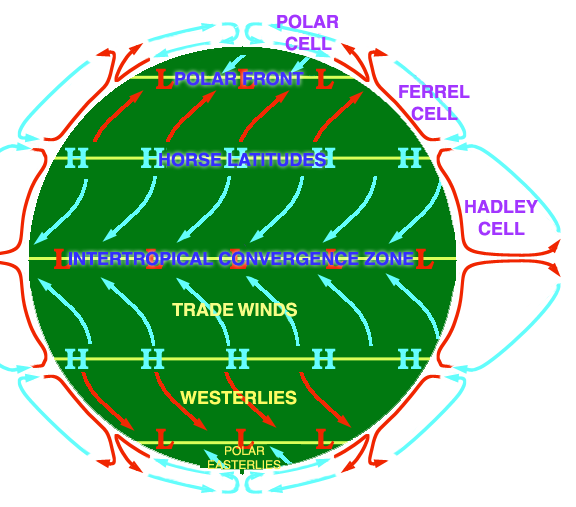
\includegraphics[scale = 0.5]{Circulacion.png}
  \caption{Figura: Circulacion atmosférica}
\end{centering}
\end{figure}

%Agregar imágen circulación

\section{Bibliografía}
\begin{verbatim}

Varios autores. (2018). Atmosphere of Earth. 2018, de Wikipedia, the free encyclopedia.
Sitio web: https://en.wikipedia.org/wiki/Atmosphere_of_Earth

\end{verbatim}
\section{Apéndice}

A continuación se presentan una serie de preguntas a responder acerca de la actividad.

\textbf{¿Qué fue lo que más te llamó la atención de esta actividad?}


El formato tan completo y formal que ofrece latex para la edición de documentos científicos.

\textbf{¿Qué fue lo que se te hizo menos interesante?}

Nada en la actividad. Todo me parecio interesante y nuevo.

\textbf{¿Qué cambios harías para mejorar esta actividad?}

Utilizaría otro tipo de ejemplo donde se incluya el uso de ecuaciones, caracteres especiales, tablas, etc. y así dominar un poco más el manejo de éste editor de texto.

\textbf{Cuál es tu primera impresión de uso de LATEX?}
En un principio parece complejo el uso del editor, sin embargo da una buena presentación a lo que es el documento finalizado.

\textbf{¿El tiempo sugerido para esta actividad fue suficiente?}

En lo personal, me hubiera hecho falta un poco más de tiempo ya que llevo acabo otras actividades y me fue difícil dedicarme unicamente a esto.

\textbf{¿Encontraste algún documento o recurso en línea útil que quisieras compartir con los demás?}

Los recursos recomendados en clase fueron de muy buen uso para mi. Recomiendo tambien la página de overleaf para edición de textos en Latex.
 
\end{document}
%configuration={"latex_command":"latexmk -pdf -f -g -bibtex -synctex=1 -interaction=nonstopmode 'Atmosphere of Earth.tex'"}